% Ohne Ko- und Kontravarianz

\section{Generics}

\begin{multicols*}{2}
\begin{itemize}
    \item Boxing / Typumwandlungen fallen weg
    \item Homogenität gewährleistet
    \item Klasse / Struct / Interface / Delegates / Events oder Methoden (auch wenn Klasse nicht generisch) können generisch sein
    \item Beliebige Anzahl generischer Typparameter erlaubt
\end{itemize}
\begin{lstlisting}
public class Buffer<TElement, TPriority> {
    TElement[] _items;
    TPriority[] _priorities;

    public void Put(TElement item, TPriority prio)
    { /* ... */ }
}
\end{lstlisting}
\subsection{Type Constraints}
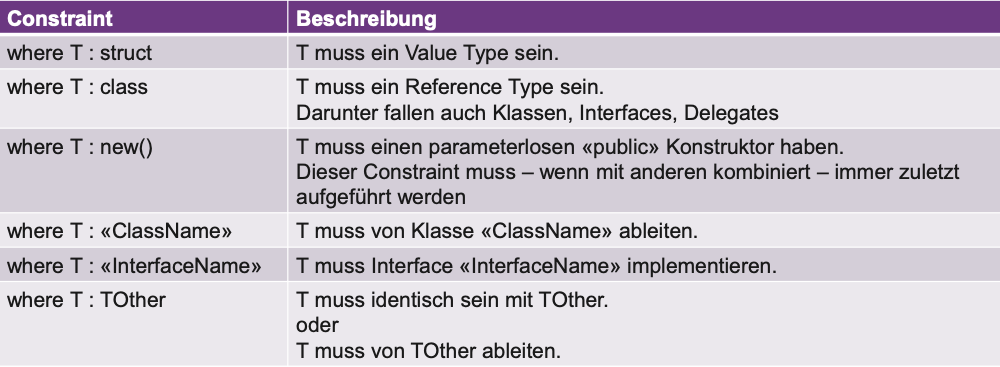
\includegraphics[width=\columnwidth]{generics}
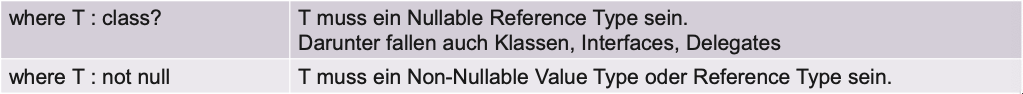
\includegraphics[width=\columnwidth]{generics2}
\fat{Beispiele:}
\begin{lstlisting}
//IComparable
class OrderedBuffer<T> where T : IComparable
{
    public bool Compare(T a, T b)
    {
        return a.CompareTo(b);
    }
}

class ExamplesCombiningConstraints<T1, T2> 
    where T1 : struct
    where T2 : Buffer,
               IEnumerable<T1>,
               new()
{
    /* ... */
}
\end{lstlisting}
\subsection{Vererbung}
Generische Klassen können von anderen generischen Klassen erben.
\begin{lstlisting}
//Normale Klassen
class MyList<T> : List { }  
//Weitergabe des Typparameters an generische Basisklasse  
class MyList<T> : List<T> { }
//Konkretisierte generische Basisklasse
class MyIntList : List<int> { }
//Mischform
class MyIntKeyDict<T> : Dictionary<int, T> { }

//Typparameter werden nicht vererbt
class MyList : List<T> { } // Compilerfehler
\end{lstlisting}
\subsubsection{Zuweisung Normale Basisklasse}
Zuweisung an Variable eines nicht-generischen Basistyps immer möglich.
\begin{lstlisting}
class MyList { }
class MyList<T> : MyList { }
class MyDict<TKey, TValue> : MyList { }

class Examples
{
    public void Test() {
        MyList l1 = new MyList<int>();
        MyList l2 = new MyDict<int, float>();
        object o1 = new MyList<int>();
        object o2 = new MyDict<int, float>();
    }
}
\end{lstlisting}
\subsubsection{Zuweisung Generische Basisklasse}
Zuweisung an Variable eines nicht-generischen Basistyps immer möglich.
\begin{lstlisting}
class MyList<T> { }
class MyList2<T> : MyList<T> { }
class MyDict<TKey, TValue> : MyList<TKey> { }

class Examples
{
    public void Test() {
        MyList<int> l1 = new MyList2<int>();
        MyList<int> l2 = new MyDict<int, float>();
        // Compilerfehler
        MyList<int> l3 = new MyList<float>();
        MyList<object> l4 = new MyList<float>();
    }
}
\end{lstlisting}
\subsubsection{Methoden überschreiben}
\begin{lstlisting}
class Buffer<T> {
    public virtual void Put(T x) { }
}

//Konkretisierte Basisklasse T wird durch int ersetzt
class MyIntBuffer : Buffer<int>
{
    public override void Put(int x) { }
}

//Generische Vererbung T bleibt generisch
class MyBuffer<T> : Buffer<T> 
{
    public override void Put(T x) { }
}
\end{lstlisting}
\subsubsection{Generic Type Inference}
Redundante Typparameter können bei Methoden weggelassen werden. Compiler erkennt Typ von Parameter automatisch.
Wenn T nur Rückgabetyp keine Erkennung.
\begin{lstlisting}
public void Test() {
    Print<int>(12);
    Print(12);

    int i1 = Get<int>();
    int i2 = Get(); // Compilerfehler
}

public void Print<T>(T t) { /* ... */ }
public T Get<T>() { /* ... */ }
\end{lstlisting}

\subsection{Generische Collections}
\begin{multicols*}{2}
\fat{Klassen:}
\begin{itemize}
    \item List<T>
    \item SortedList<TKey,TValue>
    \item Dictionary<TK,TV>
    \item SortedDictionary<TK,TV>
    \item LinkedList<T>
    \item Stack<T>
    \item Queue<T>
\end{itemize}
\columnbreak
\fat{Interfaces:}
\begin{itemize}
    \item IEnumerable<T>
    \item IEnumerator<T>
    \item ICollection<T>
    \item IList<T>
    \item IDictionary<TK,TV>
    \item IComparable<T>
    \item IComparer<T>
\end{itemize}
\end{multicols*}
\end{multicols*}